\documentclass{article}
\usepackage[utf8]{inputenc}
\usepackage[margin=1in]{geometry}
\usepackage{graphicx}
\usepackage{float}

\title{Data Structures: Problem Set 6}
\author{Jackie Luo}
\date{May 9, 2015}

\begin{document}
\maketitle

\section{Theory}

\subsection{}
a. Starting from any point in the graph, visit all of its immediate neighbors and check the number of edges from each, comparing each number of edges to the max and replacing the point to be used as the tower location if the number is greater than the max. Then, place a tower on the island found with the most neighbors and add its neighbors to a visited list. Find the next unvisited island (a neighbor of one of the last visited islands) and then repeat until each island is visited (i.e., each island can receive messages). The running time of the algorithm is O(N), as each point should only have to be visited once, and with the given map, it places two towers. The towers differ based on the start location, but if we start at A, one solution would be a tower at A, one at F, and one at J.
\newline
b. In the graph below, the greedy algorithm doesn't necessarily find the optimal solution. If we start at 0, there's a tower placed at 1, and 0 and 2 are added to the visited list. We can then place a tower at 3, add it to visited, and move to 4. We place an island at 4, add 4, 5, and 6 to the visited list, and move to 7, placing a final tower there with a total of 4. The optimal solution, however, is 3 towers (i.e., at islands 0, 2, and 6). 
\newline
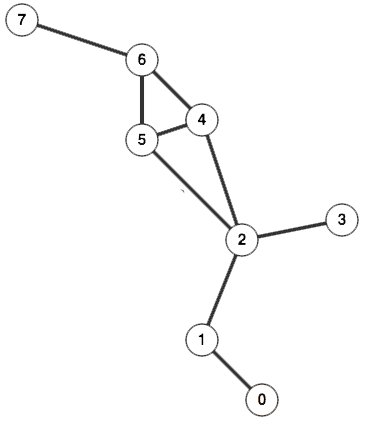
\includegraphics[scale=0.5]{map.png}
\newline
c. An algorithm that would certainly find the optimal solution for a graph could try every arrangement of towers using the same method described in the greedy algorithm, just getting every combination of its resulting placements and then returning the optimal one. To go into specifics, in the graph shown above, the naive algorithm would test placement of a tower at 0, which would add 0 and 1 to the visited list, then 2, which adds 2, 3, 4, and 5 to the visited list, then 6, which adds 6 and 7 to the visited list. That happens to result in the optimal solution on the first try, but to ensure that it is, the algorithm would continue through the graph, starting with a tower on 1, 2, 3, and so on, and going over the rest of the graph to place towers with that same principle each time.

\subsection{}
The discovery that P = NP would have the effect of rendering most cryptosystems (like public-key cryptography) ineffectual because they currently rely on the difficulty of solving NP-complete problems for their security. If it's possible for the problems to be quickly solved by computers, that would entail a major drawback to the systems that utilize them. On the flip side, it would revolutionize a lot of the existing institutions in the world by radically increasing efficiency, as problems that relate to optimization of time and/or resources would be solvable. Costs that currently are a result of non-optimal practices would be eliminated, and that change would impact the economy dramatically.

\end{document}